% TeX eps-loader file generated by McmcDiagnostics.m (Dynare).
% 08-Feb-2024 10:50:26
 
\begin{figure}[H]
\centering 
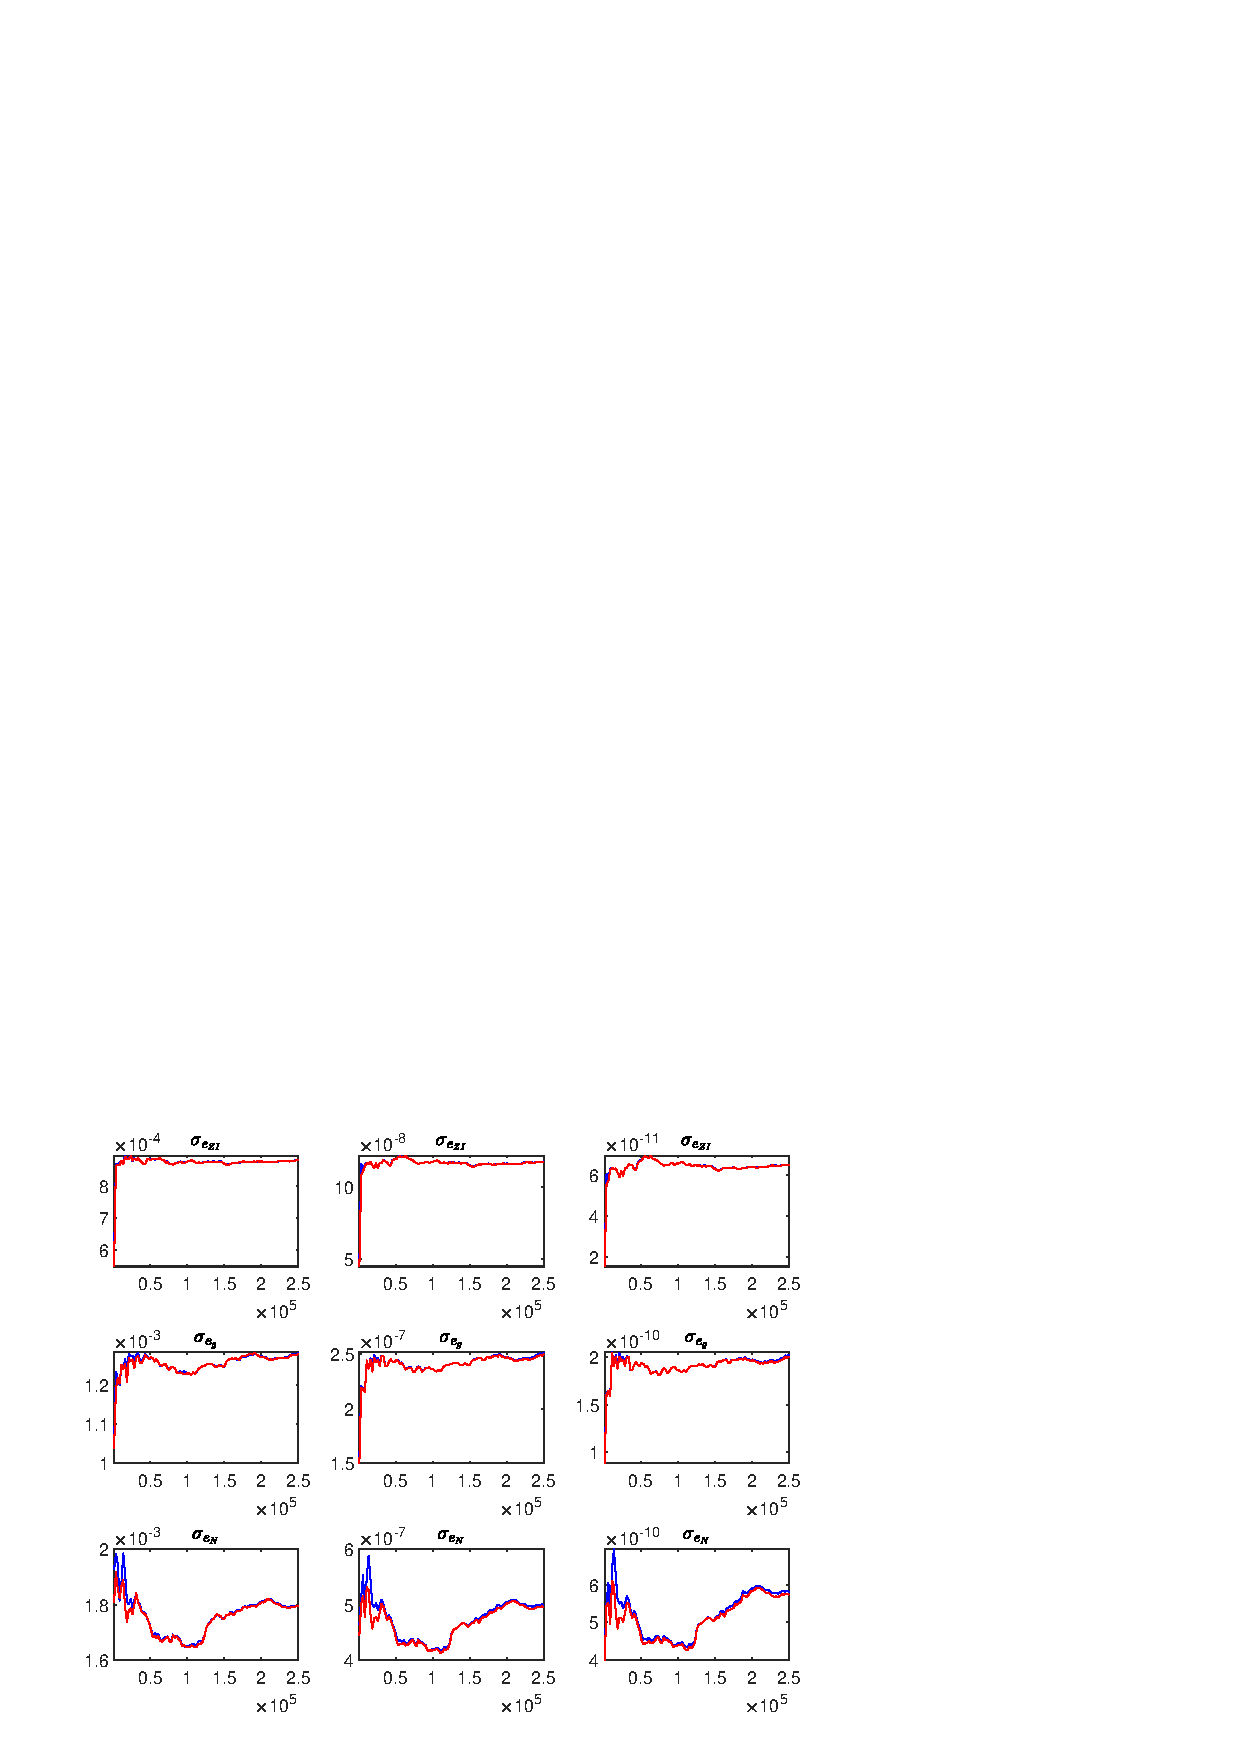
\includegraphics[width=0.80\textwidth]{BRS_imp_mobility_alt/Output/BRS_imp_mobility_alt_udiag1}
\caption{Univariate convergence diagnostics for the Metropolis-Hastings.
The first, second and third columns are respectively the criteria based on
the eighty percent interval, the second and third moments.}\label{Fig:UnivariateDiagnostics:1}
\end{figure}

\begin{figure}[H]
\centering 
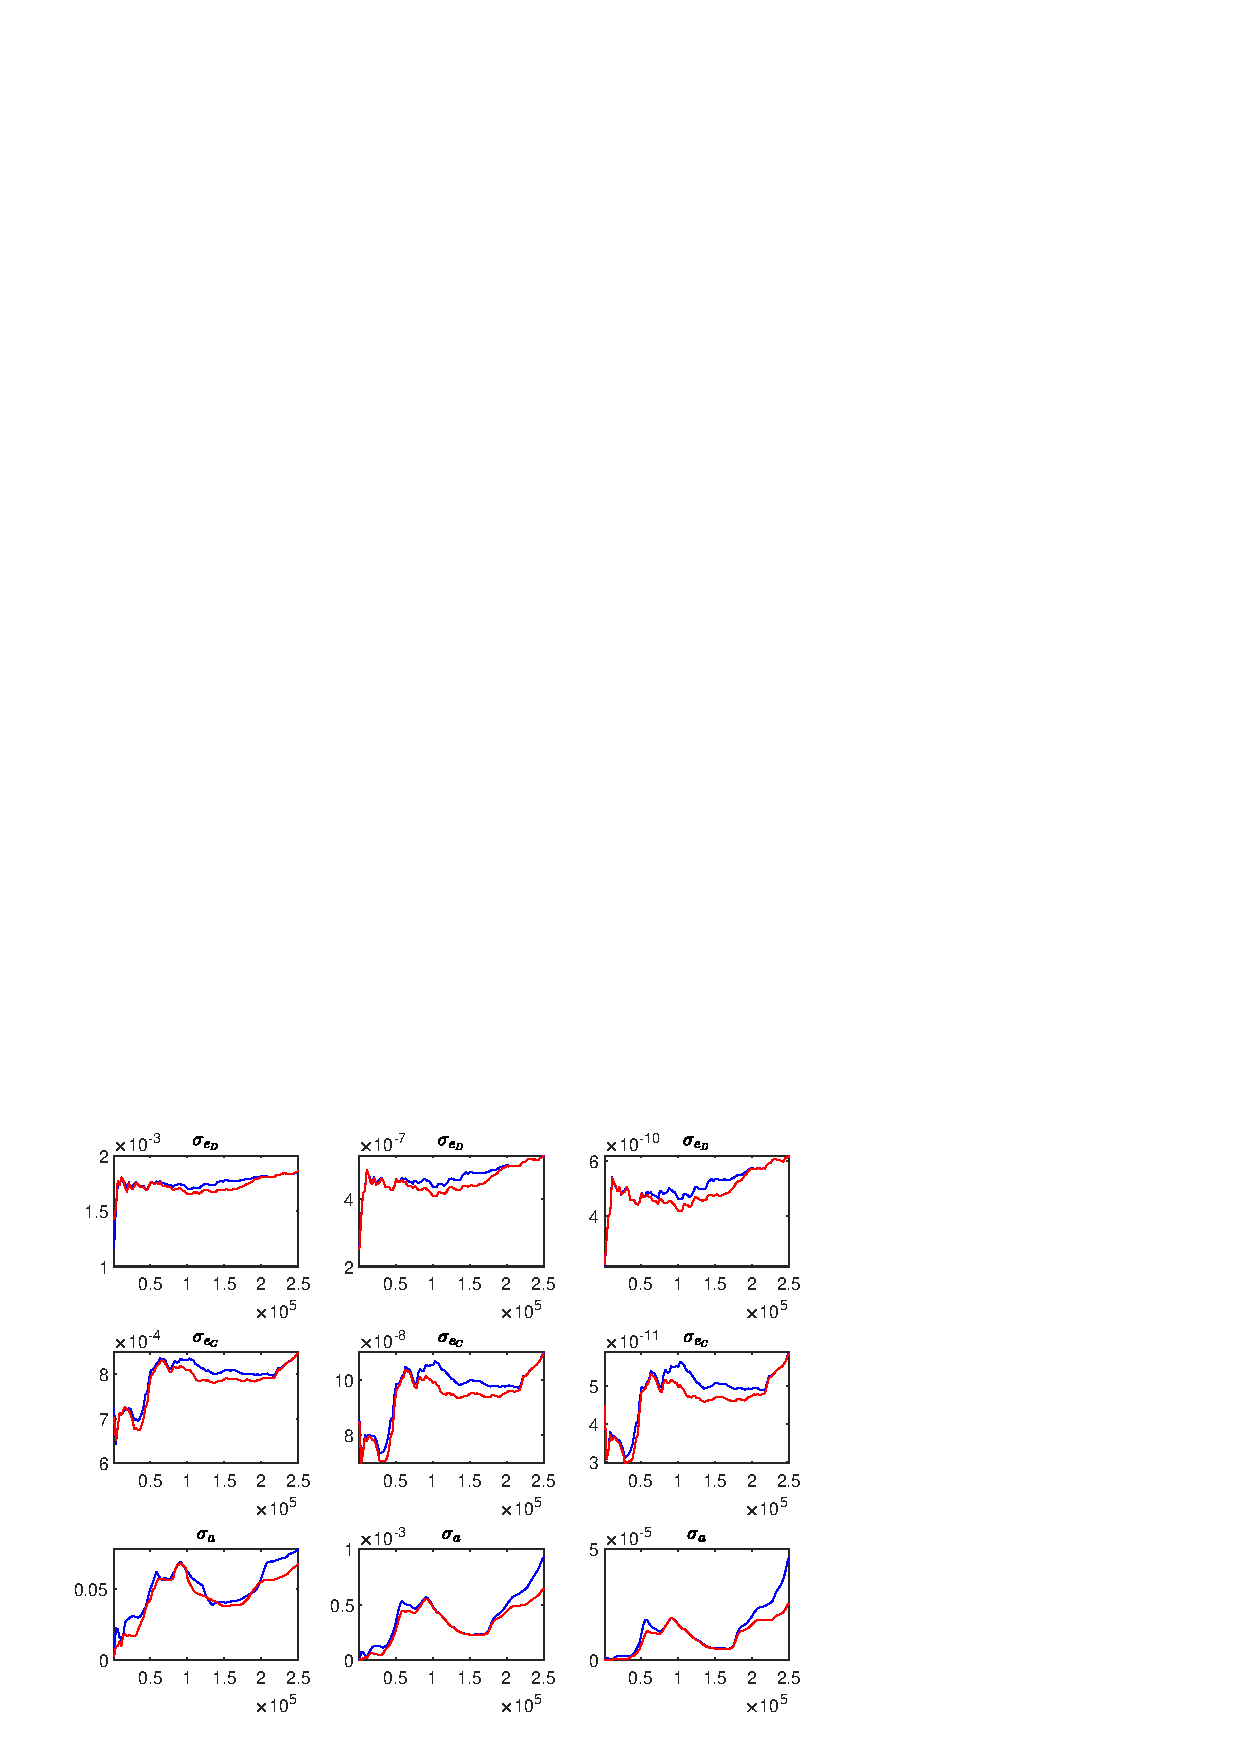
\includegraphics[width=0.80\textwidth]{BRS_imp_mobility_alt/Output/BRS_imp_mobility_alt_udiag2}
\caption{Univariate convergence diagnostics for the Metropolis-Hastings.
The first, second and third columns are respectively the criteria based on
the eighty percent interval, the second and third moments.}\label{Fig:UnivariateDiagnostics:2}
\end{figure}

\begin{figure}[H]
\centering 
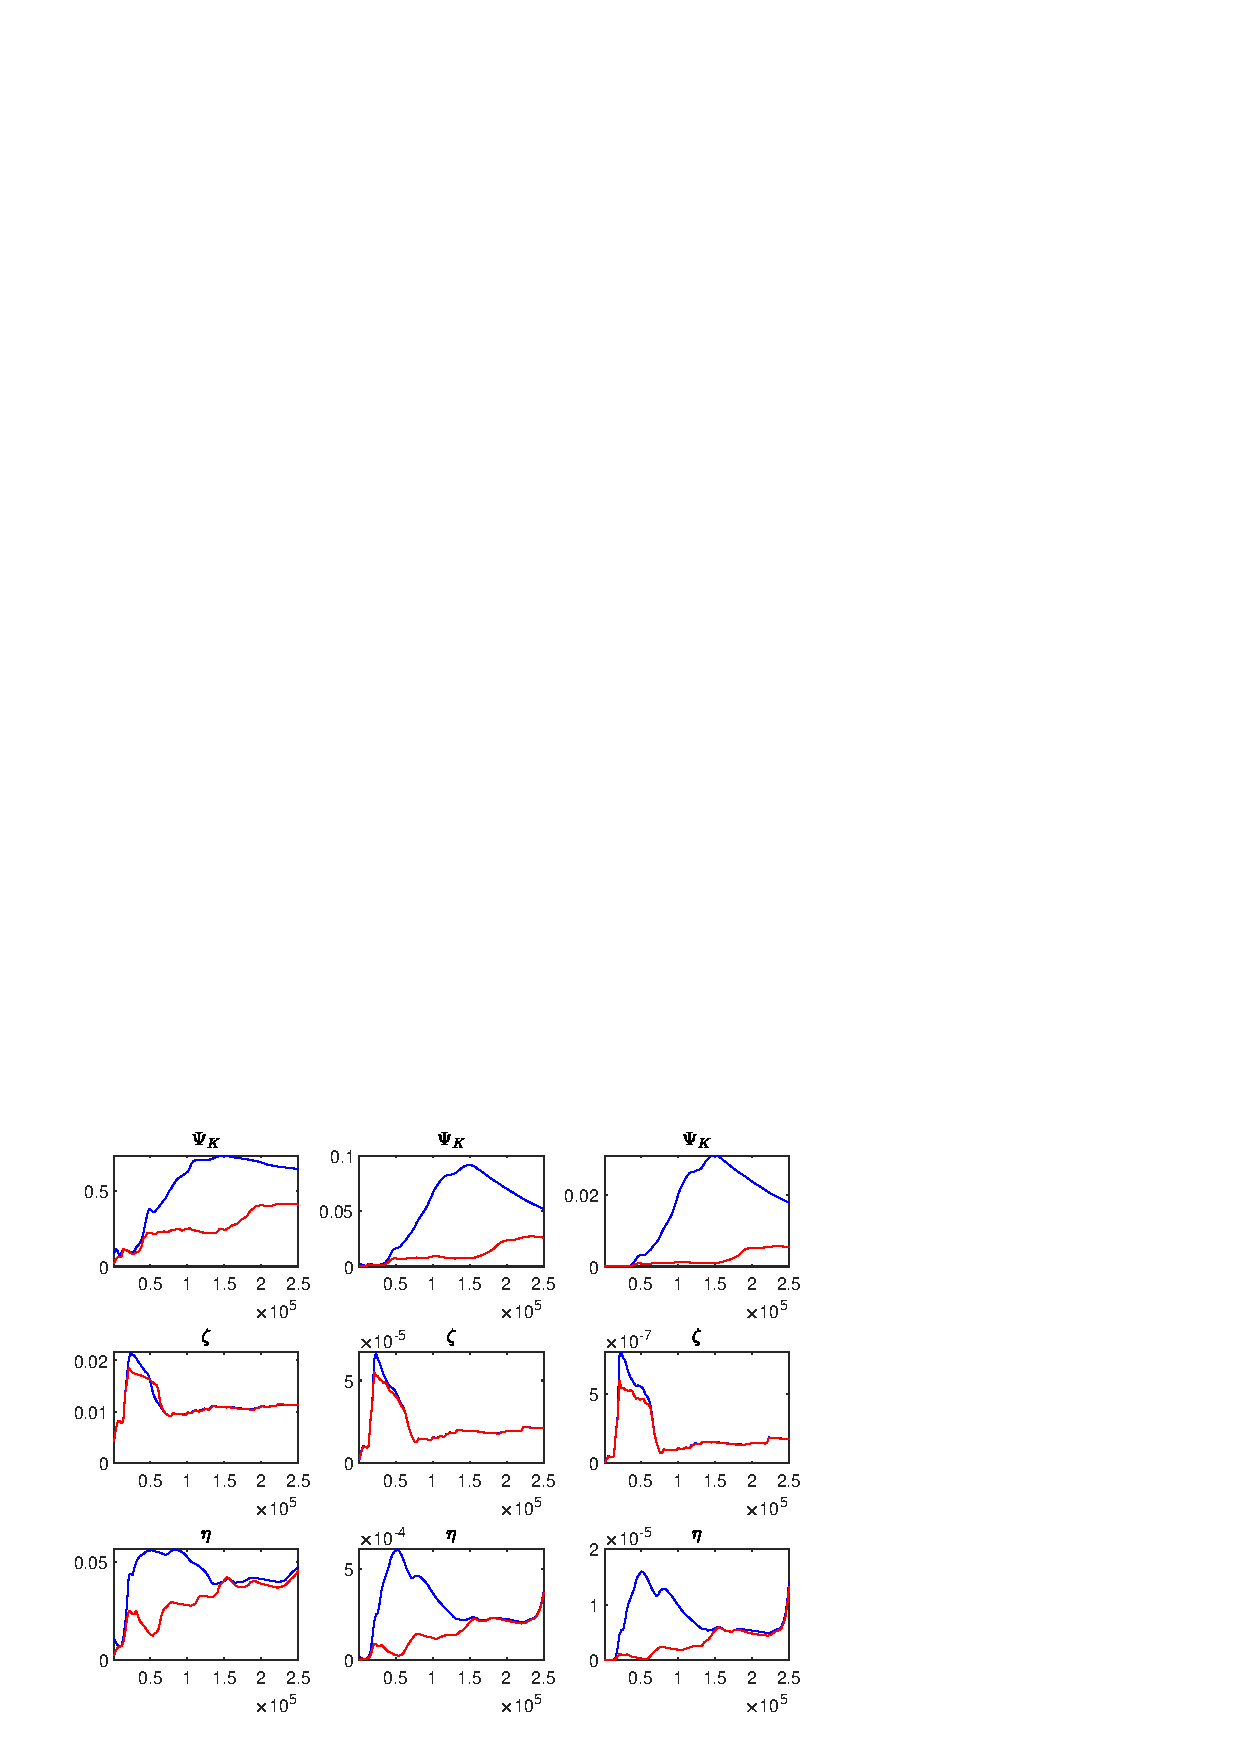
\includegraphics[width=0.80\textwidth]{BRS_imp_mobility_alt/Output/BRS_imp_mobility_alt_udiag3}
\caption{Univariate convergence diagnostics for the Metropolis-Hastings.
The first, second and third columns are respectively the criteria based on
the eighty percent interval, the second and third moments.}\label{Fig:UnivariateDiagnostics:3}
\end{figure}

\begin{figure}[H]
\centering 
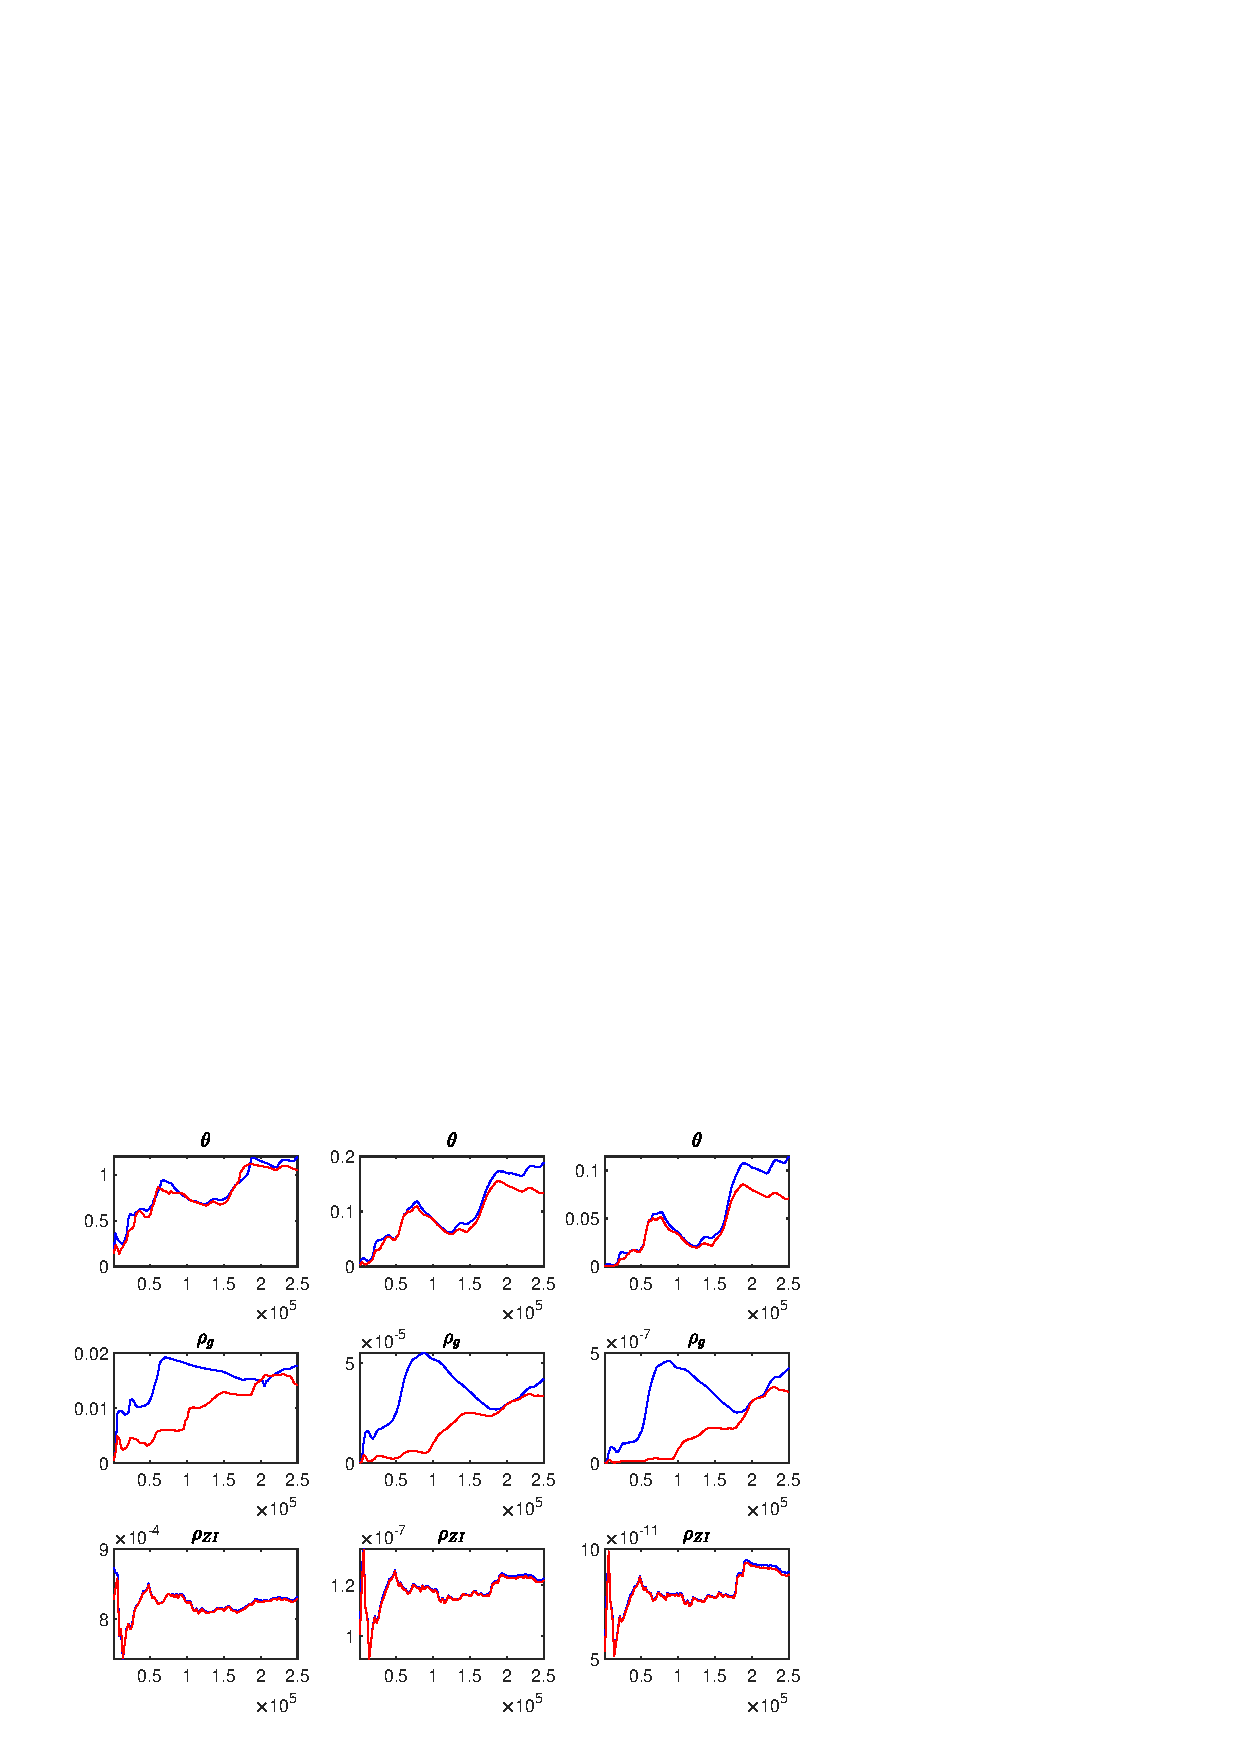
\includegraphics[width=0.80\textwidth]{BRS_imp_mobility_alt/Output/BRS_imp_mobility_alt_udiag4}
\caption{Univariate convergence diagnostics for the Metropolis-Hastings.
The first, second and third columns are respectively the criteria based on
the eighty percent interval, the second and third moments.}\label{Fig:UnivariateDiagnostics:4}
\end{figure}

\begin{figure}[H]
\centering 
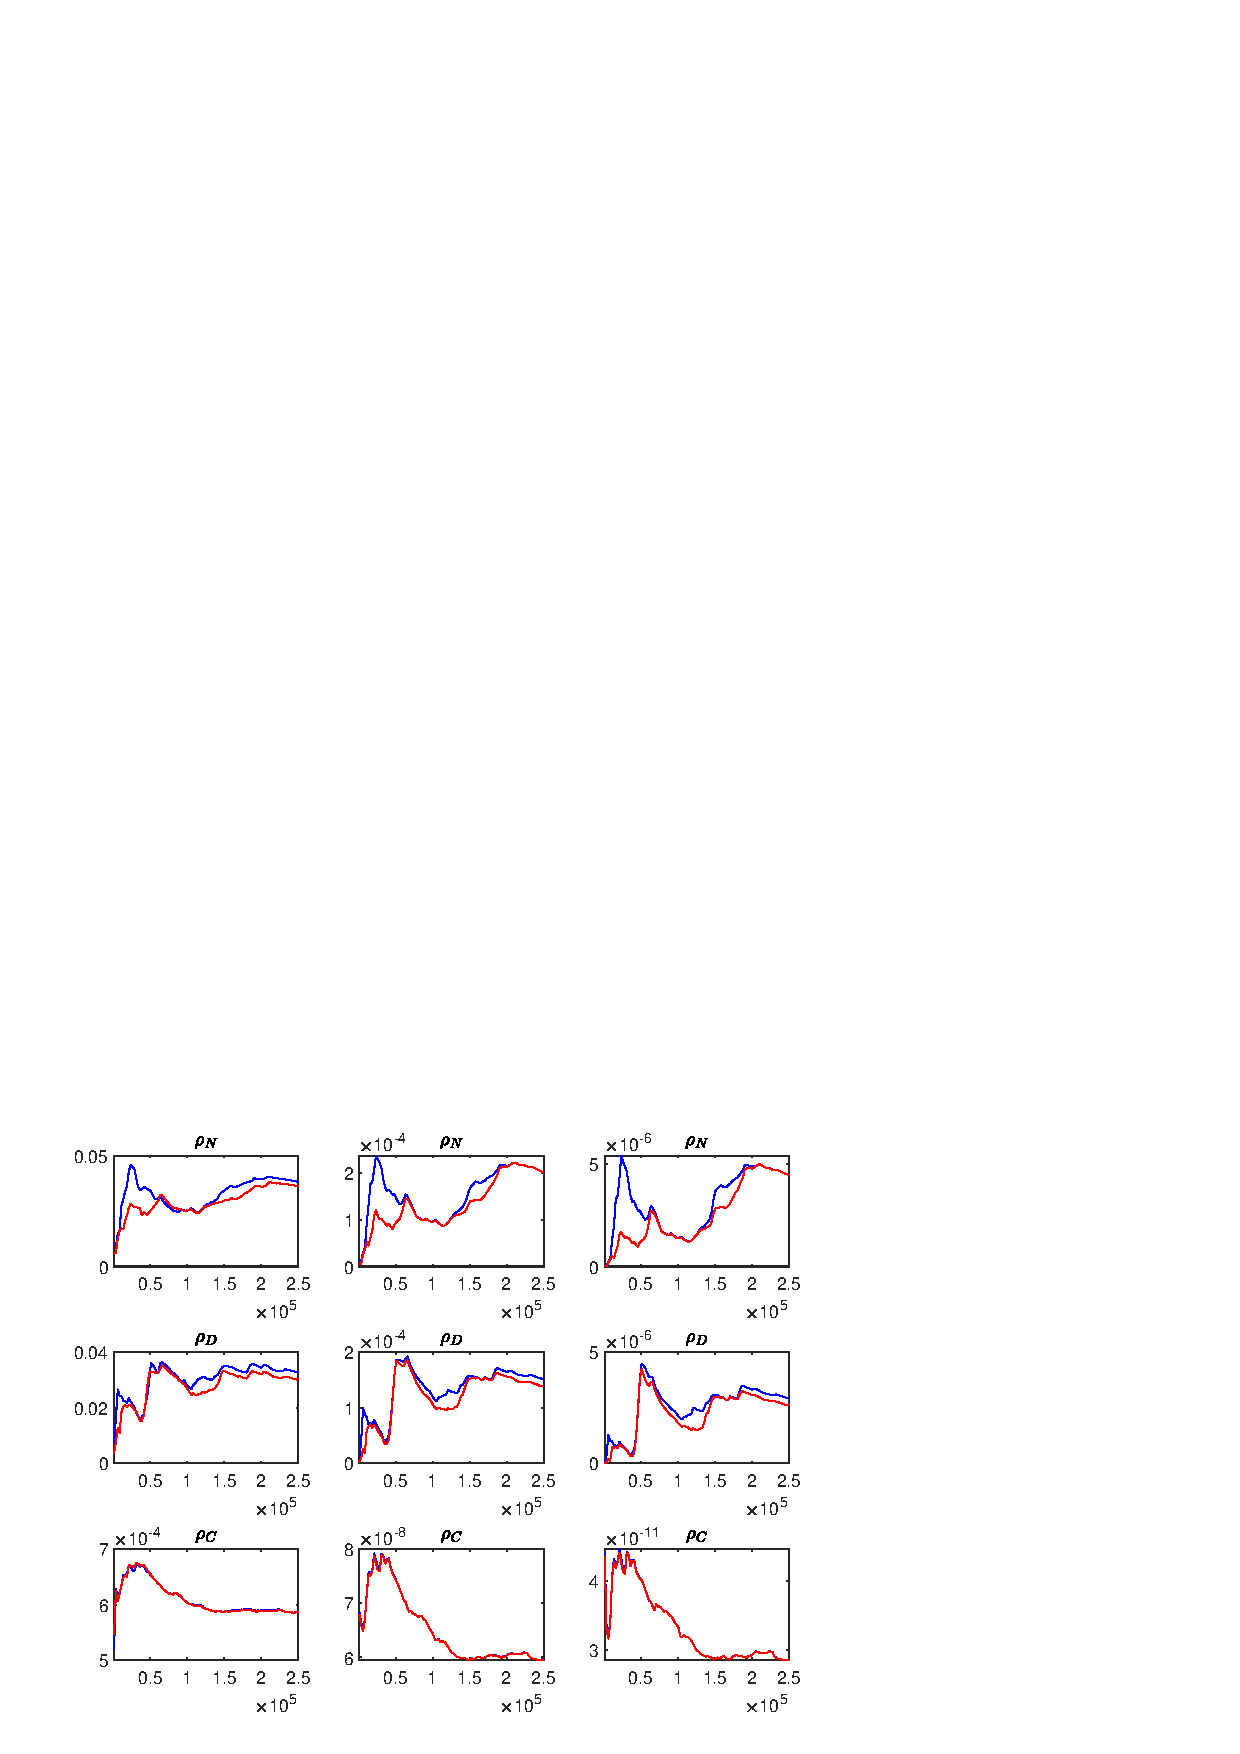
\includegraphics[width=0.80\textwidth]{BRS_imp_mobility_alt/Output/BRS_imp_mobility_alt_udiag5}
\caption{Univariate convergence diagnostics for the Metropolis-Hastings.
The first, second and third columns are respectively the criteria based on
the eighty percent interval, the second and third moments.}\label{Fig:UnivariateDiagnostics:5}
\end{figure}

